\documentclass[a4paper]{article}

\usepackage[utf8]{inputenc}
\usepackage{enumerate}
\usepackage{amssymb}
\usepackage{amsfonts}
\usepackage{amsthm}
\usepackage{amsmath}
\usepackage{graphicx}
\usepackage[ruled,vlined]{algorithm2e}
\usepackage{color}
\usepackage{xcolor,colortbl}
\usepackage{authblk}
\usepackage{hyperref}
%\usepackage{tgpagella}
\usepackage[margin=10pt,font=small,labelfont=bf,labelsep=endash]{caption}
\usepackage{abstract}
\usepackage{onecolpceurws}

%   New commands
\newcommand{\xt}{$(X_t)$ }
\newcommand{\om}{$\Omega$ }
%\renewcommand\qedsymbol{$\blacksquare$}
\renewcommand\Affilfont{\itshape\small}

%       New Environment
\newtheorem{theorem}{Theorem}
\newtheorem{lemma}{Lemma}[subsection]
\newtheorem{remark}{Remark}
\newtheorem{corollary}{Corollary}

%       Math definitions
\newcommand{\A}{\mathcal{A}}
\newcommand{\p}{\mathcal{P}}
\newcommand{\q}{\mathcal{Q}}
\renewcommand{\S}{\mathcal{S}}

%       Line numberwithin
\usepackage[left]{lineno}
%\linenumbers

%       Column color table
\definecolor{Gray}{gray}{0.85}
\definecolor{White}{rgb}{1,1,1}
\newcolumntype{a}{>{\columncolor{Gray}}c}



%\title{Random sampling of lattice polytopes using Markov chains}
\title{A Markov chain for lattice polytopes}

\author{
Julien David \\ LIPN \\
              Villetaneuse, UMR 7030 \\ david@lipn.univ-paris13.fr
\and
Lionel Pournin \\ LIPN \\
              Villetaneuse, UMR 7030 \\ pournin@lipn.univ-paris13.fr
\and
Rado Rakotonarivo \\ LIPN \\
              Villetaneuse, UMR 7030 \\ rakotonarivo@lipn.univ-paris13.fr
}

\institution{}

\begin{document}
\maketitle

\begin{abstract}
This paper describes an approach to the random sampling of lattice polytopes. The lattice polytopes we are interested in are contained in the hypercube $[0,k]^d$ and we refer to them as lattice $(d,k)$-polytopes. Our approach consists in using a Markov chain whose space of states is the set of all $d$-dimensional lattice $(d,k)$-polytopes and whose transitions add or delete vertices following simple, well-defined rules. We prove that this Markov chain provides a uniform random sampler of lattice $(d, k)$-polytopes, and give a lower bound on the mixing time when $d=2$. We also present a number of experimental results on a selection values of $k$ in dimension $d=2$.
\end{abstract}
\vskip 32pt

%{\small \noindent{\textbf{Abstract.}} This paper describes an approach to the random sampling of lattice polytopes. The lattice polytopes we are interested in are contained in the hypercube $[0,k]^d$ and we refer to them as lattice $(d,k)$-polytopes. Our approach consists in using a Markov chain whose space of states is the set of all $d$-dimensional lattice $(d,k)$-polytopes and whose transitions add or delete vertices following simple, well-defined rules. We prove that this Markov chain provides a uniform random sampler of lattice $(d, k)$-polytopes, and give a lower bound on the mixing time when $d=2$. We also present a number of experimental results on a selection values of $k$ in dimension $d=2$.}

\section{Introduction}

A polytope is the convex hull of a finite set of points in $\mathbb{R}^d$. These objects appear in a wide range of mathematical works, both in theoretical and applied contexts~\cite{ziegler1995lectures}. Yet their combinatorics is not well understood. A class of polytopes of special interest is that of \emph{lattice $(d,k)$-polytopes}. These polytopes are contained in the hypercube $[0,k]^d$, where $k$ is a positive integer, and their vertices have integer coordinates. A number of articles focus on studying their properties as a function of $d$ and $k$, even for small values of those parameters. Among these properties one finds, for instance, the maximal possible diameter of a lattice $(d,k)$-polytopes~\cite{DelPiaMichini2016,DezaManoussakisOnn2018,DezaPournin2018,KleinschmidtOnn1992,Naddef1989} which is strongly related to the Hirsch conjecture~\cite{BonifasDiSummaEisenbrandHahnleNiemeier2014,BorgwardtDeLoeraFinhold2016,KalaiKleitman1992,KleeWalkup1967,Santos2012} and, more generally, to the complexity of the simplex algorithm.

Ideally, the best way to test a conjecture would be to design an exhaustive generator of the object and perform tests up to a significant size. Unfortunately such a method is almost always unachievable in practice because the combinatorics quickly become intractable. A random sampler allows to investigate the properties of large-sized objects and the average behavior of the algorithms applied to them. Several generic methods already exist to design random generators such as the recursive method, the Boltzmann samplers, and Markov chains. The first two methods are often more efficient than the latter but they require a good knowledge of the object's combinatorics.

In this paper we present a random sampler of $d$-dimensional lattice $(d,k)$-polytopes, that is the lattice $(d,k)$-polytopes of dimension exactly $d$. The combinatorics of lattice $(d,k)$-polytopes remains elusive. For instance, there is as yet no closed formula and no asymptotic estimation for their number as a function of $d$ and $k$. Therefore, the recursive method and the Boltzmann samplers seem inapplicable at the moment for arbitrary $d$ and $k$. Note that, when $d=2$, the sampler of convex polyominoes from~\cite{bodini2013asymptotic} could be modified in order to obtain a Boltzmann sampler for lattice polygons. Also, note that in~\cite{devillers2014generator}, the authors give a random generator of convex polygons. However their setup is different from ours as they deal with polygons contained in a disc, whose vertices are not restricted to a lattice. Another easier case is when $k=1$. Indeed, any set of lattice points contained in $[0,1]^d$
is the vertex set of a lattice $(d,1)$-polytope. Thus, an ad-hoc algorithm can be easily implemented by sampling random sets of lattice points and rejecting the resulting polytopes when they are not $d$-dimensional.

The random sampler we propose results from a Markov chain, whose space of states is the set of all $d$-dimensional lattice $(d,k)$-polytopes. Its stationary distribution is uniform for any $d\geq{2}$ and positive $k$. The transitions in this Markov chain, and the resulting random sampler can be described informally as follows. Given a lattice $(d,k)$-polytope $P$ with vertex set $\mathcal{V}$, performing a transition will first consist in randomly choosing a lattice point $x$ in $[0,k]^d$, and then to proceed according to the placement of $x$ with respect to $P$. If $x$ belongs to $\mathcal{V}$, then $P$ will be replaced by the convex hull of $\mathcal{V}\mathord{\setminus}\{x\}$, thus removing $x$ from $P$. If $x$ does not belong to $\mathcal{V}$ and $\mathcal{V}\cup\{x\}$
is precisely the vertex set of its convex hull, then $P$ will be replaced by the convex hull of $\mathcal{V}\cup\{x\}$, thus inserting $x$ in $P$. If none of these two cases occurs, then $P$ will not be affected. These operations are elementary, yet they raise very interesting geometrical questions as, for instance, whether they always allow to transform any $d$-dimensional lattice $(d,k)$-polytope into any other.

In order to sample a uniform random lattice $(d,k)$-polytope, we will run a random walk on our Markov chain until we are close enough to the stationary distribution. The efficiency of the sampler is related to the time needed for the walk to get close enough to the stationary distribution. Whence, measuring the efficiency of the sampler means to determine the rate of convergence of the Markov chain to the stationary distribution as a function of the geometry and the size of the state space. Note that for several random samplers resulting form a Markov chain, estimating convergence times remains a difficult problem~\cite{carnino2011random,melanccon2001random}.

A formal definition of our Markov chain and the resulting sampler shall be given in Section~\ref{Sec.MC}. In this article we provide both theoretical and experimental results regarding the behaviour of this Markov chain. Our main result is that the random sampler built from the Markov chain for lattice $(d,k)$-polytopes is uniform. This is shown in Section~\ref{Sec.Pr}. Section~\ref{Sec.Mix} presents a general lower bound on the mixing time of our Markov chain. We conclude by giving experimental results in Section~\ref{Sec.Res}.

\section{Markov chains and random samplers}\label{Sec.MC}

We will introduce two variants of our Markov chain. The first one contains a minimal set of rules, sufficient to obtain a uniform stationary distribution. It turns out that the proof of the irreducibility of this variant raises interesting geometrical questions. The second one contains an additional rule which simplifies this proof. We provide details in Section~\ref{Sec.Pr}. For both chains, the space of states $\Omega$ is the set of all $d$-dimensional lattice $(d,k)$-polytopes, for fixed $d$ and $k$. Some effort will be needed in order to enforce the requirement that all the states of our Markov chains are polytopes of dimension exactly $d$. The transition rules of our Markov chains are defined as local operations on lattice $(d,k)$-polytopes. These rules consist in adding or removing a given vertex to such a polytope. Consider a $d$-dimensional lattice $(d,k)$-polytope $P$ and denote by $\mathcal{V}$ its vertex set. Consider a lattice point $x$ in $[0,k]^d$ which, we assume has been uniformly drawn from all possible lattice points in $[0,k]^d$. The transition from $P$ that corresponds to the chosen lattice point $x$ goes as follows.

\begin{itemize}
\item If $x$ is contained in $P$ but is not a vertex of it (i.e. $x\in{P}\mathord{\setminus}\mathcal{V}$) then the chain will loop on $P$. In other words, the current state is unaffected.
\item If $x$ is a vertex of $P$ (i.e. $x\in\mathcal{V}$), then
  \begin{itemize}
    \item If the convex hull $Q$ of $\mathcal{V}\mathord{\setminus}\{x\}$ is $d$-dimensional, the transition goes from $P$ to $Q$. Note that if $Q$ were $(d-1)$-dimensional, then $P$ would be a pyramid (with apex $x$) over $Q$. In this case, the transition from $P$ to $Q$ would be impossible because it would exit $\Omega$.
    \item Otherwise, we loop on $P$.
  \end{itemize}
  \item If $x$ does not belong to $P$, then
  \begin{itemize}
    \item If $\mathcal{V}\cup\{x\}$ is precisely the vertex set of its convex hull, then the transition goes from $P$ to the convex hull of $\mathcal{V}\cup \{x\}$.
    \item Otherwise we loop on $P$.
  \end{itemize}
\end{itemize}

Figure~\ref{fig:boucle} illustrates transition rule in the case of a lattice triangle $P$ contained in the square $[0,4]^2$, depending on the placement of point $x$. Note that in this particular case, there is no transition that deletes a vertex of $P$.

\begin{figure}[b]
  \begin{center}
    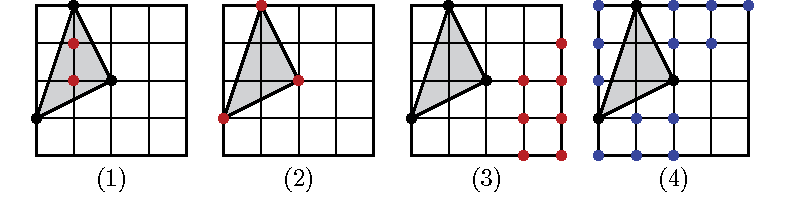
\includegraphics[scale=0.9]{../assets/boucle-mod}
    \caption{An illustration of the transition rule for a triangle (depicted in grey), depending on the placement of point $x$, colored red when the chain loops and blue when it does not loop: (1) $x$ belongs to $P\mathord{\setminus}\mathcal{V}$, (2) the convex hull of $\mathcal{V}\mathord{\setminus}\{x\}$ is $(d-1)$-dimensional, (3) $\mathcal{V}\cup\{x\}$ is not the vertex set of its convex hull, and (4) the transition changes $P$ into the convex hull of $\mathcal{V}\cup\{x\}$.}
    \label{fig:boucle}
  \end{center}
\end{figure}

By the above procedure, sampling a random lattice $(d,k)$-polytope consists in generating a random walk on the Markov chain until we are close enough to the stationary distribution. Thereby, the resulting random sampler of $(d, k)$-polytope is given by Algorithm~\ref{Algo.RS}.

\begin{algorithm}[H]\label{Algo.RS}
  \LinesNumbered
  \DontPrintSemicolon
  \KwIn{the dimension $d$, the size $k$ of the hypercube}
  \KwOut{a random lattice $(d,k)$-polytope}
  \BlankLine

  sample a random lattice $(d,k)$-simplex $P$ with vertex set $\mathcal{V}$\;
  \While{we are not close enough to the stationary distribution}{
  generate a random lattice point $x$ in $[0,k]^d$\;
  \If{$x \in \mathcal{V}$ and $\mathrm{conv}(\mathcal{V}\mathord{\setminus}\{x\})$ is $d$-dimensional}{
    $P \leftarrow \mathrm{conv}(\mathcal{V}\mathord{\setminus}\{x\})$\;
   }
  %\Else{$|\mathrm{conv}(\mathcal{V} \cup \{x\})|$ == $|\mathcal{V}| + 1$}{
  \Else{
    compute the convex hull $Q$ of $\mathcal{V}\cup\{x\}$\;
    \If{the vertex set of $Q$ is $\mathcal{V}\cup\{x\}$}{
      $P \leftarrow \mathrm{conv}(\mathcal{V} \cup \{ x\})$\;
    }
  }
 }
 \Return{$P$}
 \caption{Random sampling of a lattice $(d, k)$-polytope}
\end{algorithm}


% \begin{remark}\label{Rem.Lazy}
%   The Markov chain has been designed with the simplest rules which only consists in adding or removing vertex from a lattice $(d,k)$-polytope. However, adding more transition rules could strengthen the connectivity of the graph of the chain, thus makes it mixes faster than the primary version. Note that additional transition rules shall respect the uniformity of the resulting sampler.
%
% \end{remark}

In the other variant of our Markov chain, we introduce an additional rule when $P$ is a simplex: when the chosen random lattice point $x$ is a vertex of $P$, we may move that vertex to another lattice point instead of having a loop on $P$ in our Markov chain. More precisely, in this case we generate a new random lattice point $y$ in $[0,k]^d$ and compute the convex hull $Q$ of $[\mathcal{V}\mathord{\setminus}\{x\}]\cup\{y\}$. If $Q$ is $d$-dimensional, the transition goes from $P$ to $Q$, otherwise we loop on $P$. With this additional transition rule, we obtain Algorithm 2.

%Remark~\ref{Rem.Lazy} have us add a new transition rule: when $P$ is a simplex $x$ is chosen among vertices of $P$. If this case occurs then, instead of having a loop on $P$, we choose to move the vertex $x$ to another lattice point in $[0,k]^d$, named $y$. Then we compute the convex hull $Q$ of $\mathcal{V}\mathord{\setminus} \{x\} \cup \{y\}$. If $Q$ is $d$-dimensional, the transition goes from $P$ to $Q$, otherwise we loop on $P$. Applying this new transition rule carries out the Algorithm~\ref{Algo.RS2}.

\begin{algorithm}[H]\label{Algo.RS2}
  \LinesNumbered
  \DontPrintSemicolon
  \KwIn{the dimension $d$, the size $k$ of the hypercube}
  \KwOut{a random lattice $(d,k)$-polytope}
  \BlankLine

  sample a random lattice $(d,k)$-simplex $P$ with vertex set $\mathcal{V}$\;
  \While{we are not close enough to the stationary distribution}{
  generate random a lattice point $x$ in $[0,k]^d$\;
  \If{$x \in \mathcal{V}$}{
    \If{$|\mathcal{V}|=d+1$}{
      generate a random lattice point $y$ in $[0,k]^d$\;
      \If{$\mathrm{conv}([\mathcal{V}\mathord{\setminus}\{x\}]\cup\{y\})$ is $d$-dimensional}{
        $P\leftarrow\mathrm{conv}([\mathcal{V}\mathord{\setminus}\{x\}]\cup\{y\})$\;
      }
    }
    \ElseIf{$\mathrm{conv}(\mathcal{V}\mathord{\setminus}\{x\})$ is $d$-dimensional}{
      $P\leftarrow\mathrm{conv}(\mathcal{V}\mathord{\setminus}\{x\})$\;
    }
    %\If{$\mathrm{conv}(\mathcal{V}\mathord{\setminus}\{x\})$ is $d$-dimensional}{
      %$P\leftarrow \mathrm{conv}(\mathcal{V}\setminus\{x\})$\;
    %}
    %\Else{
      %generate random a lattice point $y$ in $[0,k]^d$\;
      %\If{$|\mathrm{conv}(\mathcal{V}\mathord{\setminus} \{x\} \cup \{y\})|$ == $d+1$}{
      %  $P\leftarrow \mathrm{conv}(\mathcal{V}\mathord{\setminus} \{x\} \cup \{y\})$\;
      %}
    }
   %}
  \Else{
    compute the convex hull $Q$ of $\mathcal{V}\cup\{x\}$\;
    \If{the vertex set of $Q$ is $\mathcal{V}\cup\{x\}$}{
      $P \leftarrow \mathrm{conv}(\mathcal{V} \cup \{ x\})$\;
    }
  }
 }
 \Return{$P$}
 \caption{Random sampling of a lattice $(d, k)$-polytope}
\end{algorithm}


The uniformity of both samplers is conditioned to the properties of the underlying Markov chains. These properties are studied in the next section.

\section{Properties of the Markov chain and uniformity of the sampler}\label{Sec.Pr}

It is well known that an irreducible, aperiodic, and symmetric Markov chain converges to the uniform for any starting distribution~\cite{levin2009markov}. In this section we prove that all these properties are satisfied by our Markov chains (reminders on their definitions will be given in the proof as well). Thus, we show that our $d$-dimensional lattice $(d,k)$-polytopes samplers are uniform.

\begin{theorem}\label{Thm.MC}
  For all $d\geq2$ and positive $k$, the Markov chain corresponding to Algorithm 1 is irreductible, aperiodic and symmetric.
\end{theorem}

\begin{proof}
  Three properties have to be verified, thus this proof will be done in three steps. Let $P$ and $Q$ be in $\Omega$, and let $\mathcal{V}$ be the vertex set of $P$.

  \begin{enumerate}[i]
    \item \textit{Irreducibility}
    A Markov chain is irreducible when all of its states can be reached from any other state. In other words the graph $\Gamma(d,k)$ underlying the Markov chain is connected. The vertex set of $\Gamma(d, k)$ is $\Omega$ and there is an edge in this graph between any two vertices that are related to one another by a single transition. The complete proof is quite involved and due to its length, we omit it here \footnote{the complete proof of the connectedness of $\Gamma(d,k)$ is provided in Appendix~\ref{sec.conect}.}. An important piece of the proof consists in showing that, given a lattice $(d,k)$-simplex $S$, there always is at least one lattice point in $[0,k]^d$ that can be inserted in $S$. It turns out that proving this seemingly simple statement is quite tricky.

    \item \textit{Symmetry}
    To prove the symmetry one needs to show that for any $P$ and $Q$, one has $\mathbb{P}(P,Q)=\mathbb{P}(Q,P)$, where $\mathbb{P}(P,Q)$ is the probability to move from $P$ to $Q$ in one step. By our transition rules, for any $P \neq Q$ we have:

    $$
      \mathbb{P}(P,Q)=\mathbb{P}(Q,P) =
      \begin{cases}
        \frac{1}{(k+1)^d}, \text{ if } \exists x \in [0,k]^d \text{ s.t. } Q=
          \begin{cases}
            \mathrm{conv}(\mathcal{V}\mathord{\setminus}\{x\})\\
            \mathrm{conv}(\mathcal{V}\cup\{x\})
          \end{cases}
        \\
        0, \text{ otherwise }
      \end{cases}
    $$

     \item \textit{Aperiodicity}
     To prove that the chain is aperiodic, one needs to show that each state in $\Omega$ has as period $1$. By definition, the period of a state $P$ is $\mathrm{gcd}(\mathcal{T}(P))$, where $\mathcal{T}(P)$ is the set of the return times in $P$. Since for an irreductible chain, all the states of $\Omega$ have the same period, then we need to find a state $P$ such that $\mathrm{gcd}(\mathcal{T}(P)) = 1$. The polytope resulting from a transition in our Markov chain must remain $d$-dimensional. In particular, if one picks any vertex of a $d$-dimensional simplex $P$, this vertex cannot be removed, and we get a loop in our Markov chain. Since there exist $d$-dimensional lattice $(d,k)$-simplices for all $d\geq2$ and positive $k$, this shows that at some state $P \in\Omega$ we have a positive probability to get back to $P$ from $P$ in one step.
     %Let $P$ be the \textit{corner simplex} of $[0,k]^d$, whose vertices are the origin (the lattice point where all coordinates are zero) and the $d$ lattice points in $[0,k]^d$ with distance $1$
     % from the origin. Then consider a point $x$ in $[0,k]^d$. The cases where we have a loop on $P$ are: either $x$ is an interior point to $P$, or $x$ is chosen outside of $P$
     % but $|Conv(\mathcal{V} \cup \{x\})| \neq |\mathcal{V}| + 1$. One has:
     % $$
     % \mathbb{P}(P,P) = \mathbb{P}\{x \  \mbox{interior point to} \ P\} + \mathbb{P}\{x \in \mathcal{V}\} + \mathbb{P}\{|\mathcal{V} \cup \{x\}| \neq |\mathcal{V}| + 1\}.
     % $$
     % Note that $\mathbb{P}\{x \in \mathcal{V}\} = \frac{d+1}{(k+1)^d}$, but since $|\mathcal{V}| = d+1$, we have a loop on $P$ with probability
     % $\mathbb{P}(P,P) \geq{ \frac{d+1}{(k+1)^d} } > 0$.
     Hence, $\mathcal{T}(P) = \{1, \dots\}$. We conclude that $\mathrm{gcd}(\mathcal{T}(P)) = 1$.

   \end{enumerate}
\end{proof}

We now prove a similar result for our modified Markov chain.

\begin{theorem}\label{Thm.Move}
  For all $d\geq2$ and positive $k$, the Markov chain corresponding to Algorithm 2 is irreductible, aperiodic and symmetric.
\end{theorem}

\begin{proof}
  We proceed the same way as we did in the proof of Theorem~\ref{Thm.MC}.

  \begin{enumerate}[i]
    \item \textit{Irreducibility}
    The proof lies on the fact that one can always find a transition path between two simplices yet the “moving a vertex” rule allows to choose one vertex of the starting simplex and move it directly to a vertex of the desired simplex. It holds as by definition a $d$-dimensional simplex is the convex hull of a set of $d+1$ affinely independant points. One can transform any $P\in\Omega$ into a simplex by consecutive deletions of its vertices, until there only remains $d+1$ of them. With an analog reasoning, by a succession of addition of vertices, we always have a transition path from a simplex to a lattice $(d,k)$-polytope. The graph of the Markov chain remains connected, hence the Markov chain is irreducible.

    \item \textit{Symmetry}
    Here the only difference from the symmetry proof in Theorem~\ref{Thm.MC} is that now we may have a one step transition between two simplices. It occurs when they only differ by a single vertex. Then, let $S$ and $S^\prime$ be two simplices in $\Omega$. If they only differ by a single vertex, then all the vertices of $S$ belong to $S^\prime$ apart from a vertex $x$, and all the vertices of $S^\prime$ belongs to $S$ apart from a vertex $y$. The probability that the transition goes from $S$ to $S^\prime$ is to choose $x$, with a $\frac{1}{(k+1)^d}$ probability, and then to move it to $y$ with a $\frac{1}{(k+1)^d}$ probability. The same argument allows to treat the transition from $S’$ to $S$. Thus,
    $$
      \mathbb{P}(S,S^\prime)=\mathbb{P}(S^\prime,S)=
      \begin{cases}
        \left(\frac{1}{(k+1)^d}\right)^2 , \text{ if } S \text{ and } S^\prime \text{ differ by a single vertex}\\
        0, \text{ otherwise}
      \end{cases}
    $$

    \item \textit{Aperiodicity}
    To prove the aperiodicity, it is necessary and sufficient to find a lattice $(d,k)$-polytope with a positive probability to loop. Let us consider a simplex $S$ with its vertices set $\mathcal{V}$ and a point $x \in [0,k]^d$. Suppose that $x$ is chosen among the vertices of $S$, then we have to redraw a point $y\in [0,k]^d$ where we decide to move $x$. The cases where we have a loop on $S$ are: either $y$ and $x$ are the same point, or $\mathrm{conv}([\mathcal{V}\mathord{\setminus}\{x\}]\cup\{y\})$ is not a $d$-simplex. Note that the probability to rechose $x$ is $\frac{1}{(k+1)^d}$.
    Then one has:
    $$
      \mathbb{P}(S,S)\geq{\frac{d+1}{(k+1)^d}\times\frac{1}{(k+1)^d}}>0.
    $$
    Thereby, $S$ has a period $1$. Since the chain is irreducible, each states of $\Omega$ has the same period $1$. The chain therefore remains aperiodic.
  \end{enumerate}
\end{proof}

It is an immediate consequence of Theorem~\ref{Thm.MC} and of Theorem~\ref{Thm.Move} that the two variations of our Markov chain have the uniform stationary distribution. Thus, the lattice $(d,k)$-polytopes obtained from both samplers are picked uniformly from $\Omega$. We have the following theorem.

\begin{theorem}\label{Thm.RS}
  The random samplers described in Algorithm~\ref{Algo.RS} and in Algorithm~\ref{Algo.RS2} are uniform random samplers for $d$-dimensional lattice $(d,k)$-polytopes.
\end{theorem}

\section{A lower bound on the mixing time}\label{Sec.Mix}

The effectiveness of the sampler is given by the number of steps it takes until one is close enough, with respect to a positive $\varepsilon < 1/2$, to the stationary distribution on $\Omega$. This quantity is called the mixing time of the Markov chain, denoted $t_{mix}(\varepsilon)$. That is, the quicker the Markov chain mixes the more effective the resulting sampler is. Obtaining an accurate estimation of the mixing time is a difficult problem. The diameter of a chain means the diameter of its graph. It refers to the longest geodesic walk on the chain between lattice $(d,k)$-polytopes. In our case, the diameter of the chain is bounded below by the difference between the largest number of vertices of a $d$-dimensional lattice $(d,k)$-polytope and the smallest number of vertices of such a polytope.

The largest number of vertices of a lattice polygon contained in a disk or a square has been studied in~\cite{AcketaZunic1995,T91,BB91}. Deza, Manoussakis and Onn have generalized this result to higher dimensions by describing lattice $(d,k)$-polytopes whose diameter are large and conjecturally maximal~\cite{DezaManoussakisOnn2018}. According to~\cite{AcketaZunic1995}, the largest number of vertices of a lattice polygon contained in $[0,k]^2$ is

\begin{equation}\label{Eqn.Deza}
  12\left(\frac{k}{2\pi}\right)^{2/3}+O(k^{1/3}\log{k})\mbox{.}
\end{equation}

We therefore immediately obtain the following lower bound on the mixing time of our sampler in the $2$-dimensional case from equation (7.3) in~\cite{levin2009markov}.

\begin{theorem}\label{Thm.Lowerbound}
When $d=2$, for any positive $k$, and for any $\varepsilon<1/2$ there exists $c>0$ such that
$$
t_{mix}(\varepsilon)\geq{ck^{2/3}}\mbox{.}
$$
\end{theorem}

For the case of higher dimensions,  B{\'a}r{\'a}ny and Larmann gave in~\cite{barany1998convex} bounds on the number of faces of each dimension of a lattice polytope contained in the the $d$-dimensional ball of radius $r$ centered at the origin as a function of $r$ and $d$. In particular they provide bounds on its number of vertices. Up to a translation and finding the right constant, Theorem 1 in~\cite{barany1998convex} also provide us the following lower bound on the mixing time.

\begin{theorem}
  For any $d\geq 2$, for any positive $k$, and for any $\varepsilon<1/2$ there exists $c_1(d)>0$ such that
  $$
  t_{mix}(\varepsilon)\geq c_1(d)k^{d \frac{d-1}{d+1}}\mbox{.}
  $$
\end{theorem}

We have carried out a number of experiments in order to get an estimation of the actual mixing time of the sampler corresponding to Algorithm~\ref{Algo.RS} in the $2$-dimensional case. These results are presented in Section~\ref{Sec.Res}.

%Deza, Manoussakis and Onn have studied a class of $(d,k)$-polytope which has the maximal number of vertices in~\cite{DezaManoussakisOnn2018}. If we consider a lattice $(d,k)$-polytope and note by $\delta(d,k)$ its diameter. They found the maximal diameter of a lattice $(2,k)$-polytope (i.e. a lattice convex polygon), as a function of $k$. They proved that:

%Questions about the maximal diameter of lattice polygons has been focused the last two decades by several searchers. Here the diameter of is defined as the diameter of the graph which has as set of vertices the vertices of the polygon and as edges, its edges. For the lattice $(d,k)$-polytope, this diameter is denoted by $\delta(d,k)$. Deza, Manoussakis and Onn found in~\cite{DezaManoussakisOnn2018} the maximal diameter of a lattice $(2,k)$-polytope, as a function of $k$. They proved that:


%The lattice polygons which realizes this maximal diameter possesses the maximal number of vertices as well. This maximal number of vertices, noted $N_{max}$, satisfies the relation:
%\begin{equation}\label{Eqn.Nmax}
%  \delta(2,k) = \left\lfloor \frac{N_{max}}{2} \right\rfloor.
%\end{equation}

%Given equation (\ref{Eqn.Deza}) and equation (\ref{Eqn.Nmax}), we obtain the an upper bound on the mixing time.

%\begin{theorem}
%  For $d=2$ and for all $k$. We have:
%  \begin{equation}
%    t_{mix}\leq{ck^{\frac{2}{3}}} \ \mbox{with} \ c>0.
%  \end{equation}
%\end{theorem}

%A number of experiments has been done on our chain in order to estimate the actual mixing time according to our theoretical upper bound. Those results are presented in Section~\ref{Sec.Res}.

\section{Experimental results}\label{Sec.Res}

The empirical estimations we conduct are based on the \textit{ergodic theory} and on the \textit{coupling} method on Markov chains. Applying the ergodic theory on Markov chains requires the irreducibilty and the positive recurrency of the chain, properties we verified on our model since we have a finite space of states~\cite{levin2009markov}. The ergodic theory states that for any real-valued function on the states, its average value, for a long enough  walk on our chain, is the same as the expectancy at the stationary distribution, see Theorem 4.16 in~\cite{levin2009markov}. Here the function can be any quantity we can measure on lattice $(d,k)$-polytopes. The process is the following: we run a long walk on the Markov chain, evaluate the quantity on each state we visit, then calculate the average value of this quantity over the whole run. By the ergodic theory we are able to estimate average properties on our objects with an enough long walk on our chain.

We chose to measure two quantities on our lattice polygons in order to get estimations of the mixing time via the ergodic theory: the number of vertices and the area. We measured these quantities on walks with respectively 1000, 10000, and 100000 steps for $3\leq{k}<100$. Then we compare the average measures for the two latter quantities in different length walks in Figure~\ref{Fig.NV}\footnote{we provide more detailed results in Table~\ref{Tab.Summary} in Appendix~\ref{Sec.Tab}.}. For $k\leq 20$, observe that the average values of the number of vertices and the area of a polygon seems to stabilize, implying that the time needed by the chain to mix is less than 100000 steps. For greater values of $k$ we measured the average values in a 1 million step walk, in order to have an idea on the time the average values will stabilize. The results are shown in Table~\ref{Tab.Cmp}. Observe in the four last rows of Table~\ref{Tab.Cmp} that the behaviour of the average number of vertices of a polygon and its average area does not vary anymore when we reach 1 million steps, compared to the 100000 steps walk. Given those figures we can make the following observations, when the number of steps $t\geq 1000000$:

\begin{equation}
  \mathbb{E}_\pi[n_t] \sim 2k^{2/3} \text{ and } \mathbb{E}_\pi[v_t] \leq 0.68k^2.
\end{equation}

where $\mathbb{E}_\pi[n_t]$ and $\mathbb{E}_\pi[v_t]$ are respectively the expectancy of the number of vertices and the area of a polygon at the stationary distribution $\pi$ \footnote{figures are given to see the estimation as a function of $k$ in Figure~\ref{Fig.Nlim} and Figure~\ref{Fig.Vlim} in Appendix~\ref{Sec.Tab}.}.

% average number of vertices
\begin{figure}[t]
  \begin{center}
    \begin{minipage}[c]{.45\linewidth}
      \includegraphics[scale=.4]{npoint}
    \end{minipage}
    \begin{minipage}[c]{.45\linewidth}
      \includegraphics[scale=.4]{volume}
    \end{minipage}
    %\includegraphics[scale=0.6]{npoint.eps}
    \caption{For $3\leq{k}<100$, compared average measures in a long run with respectively $1000$, $10000$ and $100000$ steps. On the left, the average number of vertices of a polygon. On the right, the average area of a polygon.}
    \label{Fig.NV}
  \end{center}
\end{figure}

%comparison for k>=20
\begin{table}[t]
  \centering
  \begin{tabular}{c|c|c|c|c|a|a|a|a}
    & \multicolumn{2}{c|}{$1000$ steps} & \multicolumn{2}{c|}{$10000$ steps} & \multicolumn{2}{c|}{$100000$ steps} & \multicolumn{2}{c}{$1$ million steps}\\
    \hline
    \hline
    \rowcolor{White}
    $k$ & $\bar{n}$ & $\bar{v}$ & $\bar{n}$ & $\bar{v}$ & $\bar{n}$ & $\bar{v}$ & $\bar{n}$ & $\bar{v}$ \\
    \hline
    20 & 13.07 & 209.562 & 14.170 & 219.586 & 13.929 & 246.689  & 14.101 & 249.485\\
    30 & 13.501 & 356.220 & 16.835 & 532.784 & 18.165 & 585.092 & 18.162 & 603.668\\
    40 & 14.904 & 365.466 & 20.393 & 714.765 & 22.618 & 855.234 & 22.041 & 1021.824\\
    50 & 18.875 & 369.500 & 21.639 & 816.006 & 25.351 & 1779.055 & 25.909 & 1437.172\\
    60 & 18.813 & 542.450 & 20.51 & 1112.126 & 27.56 & 2337.680 & 27.419 & 2452.580\\
    70 & 17.534 & 525.187 & 21.804 & 1271.738 & 31.058 & 3022.452 & 30.674 & 2978.699\\
    80 & 18.8 & 593.20 & 24.999 & 1547.383 & 32.995 & 3343.108 & 32.429 & 3310.488\\
    90 & 19.771 & 562.75 & 24.240 & 1499.416 & 33.903 & 3728.283 & 33.836 & 3722.788\\
    \hline
  \end{tabular}
  \caption{For large value of $k$. Detailed values of the average number of vertices~$\bar{n}$ of a polygon and the average area~$\bar{v}$ of a polygon in a long walk on the chain.}
  \label{Tab.Cmp}
\end{table}

The coupling method is another way to estimate the mixing time. The coupling is more general and often used to bound rates of convergence to stationarity as well. It consists in running two walks, with different distribution, on the Markov chain. The coupling result on Markov chains tells us that once two coupled walks are at the same state, they will both move following the stationary distribution. Though, this gives us little information about the actual time the walk reaches the stationary distribution. Note that the walk may have reached the stationary distribution earlier. Our computations allowed us to get an empirical upper bound on the  mixing time in the $2$-dimensional case for $k$ up to $6$, the computation time becoming prohibitive for larger values of $k$. Table~\ref{Tab.Coupling} presents execution times for this method and the number of steps needed for the two walks to meet.

\begin{table}[t]
  \centering
  \begin{tabular}{c|r|r}
    $k$ & Number of steps & Execution time\\
    \hline
    \hline
    1 & 2 & 0.001s \\
    2 & 5026 & 0.164s \\
    3 & 42247 & 1.368s \\
    4 & 11387661 & 6m11s \\
    5 & 78745909 & 42m45s \\
    6 & $3.928 \times 10^9$ & 2133m20s \\
    %7 & $7.8 \times 10^8$ & 3906m31s \\
    \hline
  \end{tabular}
  \caption{Time needed to reach the stationary distribution with two coupled walks. The first starting at the corner simplex $S=\{(0,0),(1,0),(0,1)\}$ and the second at its opposite corner simplex $S^\prime=\{(k,k-1),(k-1,k),(k,k)\}$.}
  \label{Tab.Coupling}
\end{table}

%In addition we compare our results on the maximal number of vertices of a polygon to the result in equation (\ref{Eqn.Deza}) in Table~\ref{Tab.Max}. We ran a long walk on our Markov chain which number of steps of  were chosen according to the approximated number of steps we obtained in Table~\ref{Tab.Coupling}. For $k\geq{7}$, we ran a $100000$ steps walk.

% \begin{table}[Hb]
%   \centering
%   \begin{tabular}{|c|c|c|c|}
%     \hline
%     $k$ & $\delta(2,k)$ & $\delta'(2,k)$ & $N_{max}$  \\
%     \hline
%     1 & 2 & 2 & 4 \\
%     2 & 3 & 3 & 6 \\
%     3 & 4 & 4 & 8 \\
%     4 & 4 & 4 & 9 \\
%     5 & 5 & 5 & 10 \\
%     6 & 6 & 6 & 12 \\
%     7 & 6 & 6 & 12 \\
%     8 & 7 & 6 & 13 \\
%     9 & 8 & 7 & 14 \\
%     10 & 8 & 7 & 15 \\
%     11 & 8 & 7 & 15 \\
%     12 & 9 & 8 & 16 \\
%     13 & 10 & 8 & 17 \\
%     14 & 10 & 8 & 17 \\
%     15 & 10 & 9 & 19 \\
%     16 & 11 & 9 & 19 \\
%     17 & 12 & 9 & 19 \\
%     \hline
%   \end{tabular}
%   \caption{The maximal diameter $\delta'(d,k)$ of a polygon we obtain compared to the results of Deza, Manoussakis and Onn in~\cite{DezaManoussakisOnn2018}. For $k\in[1,6]$, $\delta'(d,k)$ was calculated according to the largest polygon a walk reaching the stationnary distribution visited. For $k\geq{7}$ we ran a $100000$ steps walk.}
%   \label{Tab.Max}
% \end{table}

%\begin{table}[]
%  \centering
%  \begin{tabular}{c|ccccccccccccc}
%    $k$ & 1 & 2 & 3 & 4 & 5 & 6 & 7 & 8 & 9 & 10 & 11 & 12 & 13\\
%    \hline
%    \hline
%    $\delta(2,k)$ & 2 & 3 & 4 & 4 & 4 & 5 & 6 & 7 & 8 & 8 & 8 & 9 & 10\\
%    $\delta'(2,k)$ & 2 & 3 & 4 & 4 & 5 & 6 & 6 & 6 & 7 & 7 & 7 & 8 & 8 \\
%    $N_{max}$ & 2 & 6 & 8 & 9 & 10 & 12 & 12 & 13 & 14 & 15 & 15 & 16 & 17\\
%    \hline
%  \end{tabular}
  %\caption{The maximal diameter $\delta'(d,k)$ of a polygon we obtain compared to the results of Deza, Manoussakis and Onn in~\cite{DezaManoussakisOnn2018}. For $1\leq{k}\leq{6}$, $\delta'(d,k)$ was calculated according to the largest polygon a walk reaching the stationnary distribution visited. For $k\geq{7}$ we ran a $100000$ steps walk.}
  %\caption{The maximal number of vertices of visited polygon in a long run, $N_{max}$, compared to the result in equation~(\ref{Eqn.Deza}).}

%  \label{Tab.Max}
%\end{table}

%\clearpage

% \section{Discussions and further works}
% For now our implementation is still restricted in dimension $d=2$ and struggles to reach great values of $k$. We only have reliable results for $k \in [1,6]$, since the chain hardly mixes for greater values. However the sampler resulting from the Markov chain is uniform for all $k$ and $d$. On going works is looking at the case of the dimension $d\geq{3}$, we are confident to get better result in dimension $d=3$. We strongly think that the mixing time for the Markov chain is only exponential as a function of $k$ but not in $d$. Even for small values of $k$, since in dimension $d=3$, a bound to the maximal diameter is only known for $k\leq{3}$~\cite{DezaManoussakisOnn2018}.
%
% Proving the irreducibility of the Markov chain has rised an iterresting question, as it lies on the connexity of the graph of the chain. The question was the possibility to connect two lattice $(d,k)$-polytopes by a sequence of lattice $(d,k)$-polytopes such that two consecutive polytopes in that sequence only differs by a single vertex. And we can obtain the next lattice $(d,k)$-polytope in the sequence by either add or delete a vertex from the previous. Under the assumption that we only want a sequence of $d$-dimensional $(d,k)$-polytope, proving the connectivity of the graph has been slightly tricky and is detailed in [refToLongPaper]. Always related to the connectivity of this graph and in dimension $d=2$, if lattice $(d,k)$-simplices only allow the addition of a vertex, in opposition to them there exists a family of lattice $(d,k)$-polytopes that only allow deletions. Does this family holds in $d\geq{3}$? And if it does, does it exist a value of $k$ for which such polytopes does not appear anymore? This family seems to have a particular interest in the topology of the graph. Figures~\ref{Fig.Del} illustrates examples of this family.

% \begin{figure}
%   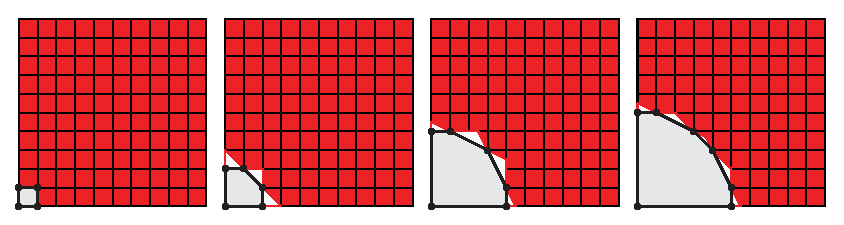
\includegraphics[width=\textwidth]{../assets/odd}
%   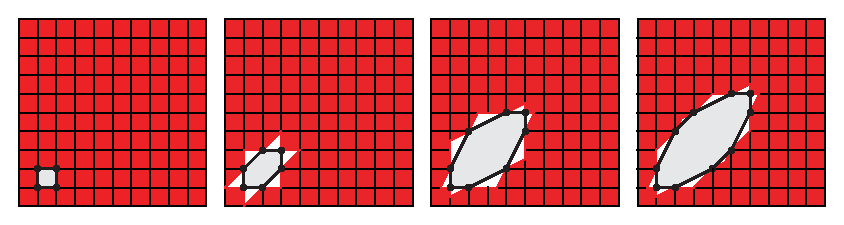
\includegraphics[width=\textwidth]{../assets/even}
%   \caption{In opposition to simplices, these lattice $(d,k)$-polytopes only allow deletion of a vertex.}
%   \label{Fig.Del}
% \end{figure}


\bibliographystyle{plain}
\bibliography{biblio.bib}

\clearpage

\appendix

\section{The insertion move for lattice simplices}\label{sec.insert}

Consider a $d$-dimensional lattice simplex $S$ contained in $[0,k]^d$, where $d\geq2$ and $k\geq1$. Let $\mathcal{V}$ be the set of vertices of $S$. For any vertex $u\in\mathcal{V}$, denote by $H_u$ the affine hull of the facet of $\S$ opposite $u$, and by $H_u^-$ the closed half-space of $\mathbb{R}^d$ limited by $H_u$ that does not contain $u$.
For any $v\in\mathcal{V}$, the intersection
\begin{equation}
  C_v=\bigcap_{\substack{u\in\mathcal{V}\\u\neq{v}}}H_u^-
\end{equation}
is a $d$-dimensional cone pointed at $v$. This cone is exactly the set of the points $x\in\mathbb{R}^d$ such that the convex hull of $S\cup\{x\}$ does not admit $v$ as a vertex. By this remark, we have the following lemma.

\begin{lemma}\label{Lem.A}
Let $x$ be a lattice point in $[0,k]^d$. The convex hull of $S\cup\{x\}$ admits $\mathcal{V}\cup{x}$ as its vertex set if and only if $x$ does not belong to $S$ and, for every vertex $v\in\mathcal{V}$, $x$ does not belong to $C_v$.
\end{lemma}

For any $i\in\{1, ..., d\}$, call
$$
\gamma_i^-=\min\{x_i:x\in{S}\}\mbox{ and }\gamma_i^+=\min\{x_i:x\in{S}\}\mbox{.}
$$

Note that, for all $i\in\{1, ..., d\}$, $\gamma_i^-<\gamma_i^+$ because $S$ is $d$-dimensional. The following is the smallest $d$-dimensional combinatorial hypercube containing $S$, whose facets are parallel to the facets of $[0,k]^d$:
$$
Q=\prod_{i=1}^d[\gamma_i^-,\gamma_i^+]
$$

Consider a facet $R$ of $Q$. The intersection of $R$ and $S$ is a non-empty, proper face $F$ of $S$. Since $S$ is a simplex, it admits another non-empty face $F^\star$ whose vertices are exactly the vertices of $S$ that do not belong to $F$.

By construction,
$$
\mathrm{dim}(F)+\mathrm{dim}(F^\star)=d-1\mbox{.}
$$

In particular, there exists a vector $c$ that is orthogonal to both $F$ and $F^\star$. Consider the hyperplane $Y$ of $\mathbb{R}^d$ that admits $c$ as a normal vector and such that $F^\star\subset{Y}$. The intersection $S\cap{Y}$ is precisely $F^\star$. Denote by $Y^-$ the closed half-space of $\mathbb{R}^d$ bounded by $Y$ that does not contain $F$. In the statement of the following lemma, $\mathrm{aff}(F)$ denotes the affine hull of $F$.

\begin{lemma}\label{Lem.B}
Consider a vertex $v$ of $S$.
\begin{itemize}
\item[i.] If $v$ is a vertex of $F$, then $C_v\cap{Q}$ is a subset of $\mathrm{aff}(F)$,
\item[ii.] If $v$ is a vertex of $F^\star$, then $C_v$ is a subset of $Y^-$.
\end{itemize}
\end{lemma}

\begin{proof}
First observe that, if $s$ is a face of $S$ and $H$ is a hyperplane of $\mathbb{R}^d$ that intersects $S$ exactly along $s$, then
$$
\bigcap_{\substack{u\in\mathcal{V}\\u\not\in{s}}}H_u^-\subset{H^-}\mbox{,}
$$
where $H^-$ is the closed half space of $\mathbb{R}^d$ bounded by $H$ and disjoint from the interior of $S$. Further observe that the intersection of $H$ with
$$
\bigcap_{\substack{u\in\mathcal{V}\\u\not\in{s}}}H_u^-
$$
is precisely the affine hull of $s$. Taking $s=F$ and $H=\mathrm{aff}(R)$, one obtains that for any vertex $v$ of $F$, $C_v\cap{Q}$ is a subset of $\mathrm{aff}(F)$. Taking $s=F^\star$, and $H=Y$, ones obtains that, for any vertex $v$ of $F^\star$, $C_v$ is a subset of $Y^-$.% The result therefore holds because any vertex of $\S$ is either a vertex of $F$ or a vertex of $F^\star$.
\end{proof}

As an immediate consequence of this and Lemma \ref{Lem.A}, for any lattice point $x\in[0,k]^d$ that does not belong to the affine hull of $F$, or to $Y^-$, the convex hull of $S\cup\{x\}$ admits, as vertices, $x$ and all the vertices of $S$.

Assume, without loss of generality that $c$ has norm $1$ and that it points towards $Y^-$. Observe that the intersection of $[0,k]^d$ with the affine hull of $R$ is a $(d-1)$-dimensional cube. Denote
\begin{equation}\label{eq.A}
\delta=\min\{c\mathord{\cdot}x:x\in\mathrm{aff}(R)\cap[0,k]^d\}\mbox{.}
\end{equation}

The set
$$
G=\{x\in\mathrm{aff}(R)\cap[0,k]^d:c\mathord{\cdot}x=\delta\}
$$
is a face of $\mathrm{aff}(R)\cap[0,k]^d$. It follows that $G$ is a cube of dimension at most $d-1$. Recall that $c$ is orthogonal to both $F$ and $F^\star$. As a consequence, the map $x\mapsto{c\mathord{\cdot}x}$ is constant within $F$ and within $F^\star$. Call $\varepsilon$ the value of $c\mathord{\cdot}x$ when $x\in{F}$ and $\varepsilon^\star$ the value of $c\mathord{\cdot}x$ when $x\in{F^\star}$. Since $F$ and $Y^-$ are disjoint, $\varepsilon<\varepsilon^\star$. Moreover, by (\ref{eq.A}), $\delta\leq\varepsilon$. Observe that the latter inequality is strict if and only if $F$ is not a subset of $G$. In this case, $F$, $G$, and $Y$ belong to distinct parallel hyperplanes and we immediately obtain the following.
\begin{lemma}\label{Lem.BC}
If $F\not\subset{G}$ then $G$ is disjoint from both $\mathrm{aff}(F)$ and $Y^-$.
\end{lemma}

If, on the contrary, $\delta$ and $\varepsilon$ coincide, then $F\subset{G}$. This situation is familiar: we are looking at a lattice simplex $F$ contained in a (possibly degenerate) lattice cube $G$. If the dimension of $G$ is greater than the dimension of $F$, then the following lemma provides the desired result.

\begin{lemma}\label{Lem.C}
If $k$ and $d$ are positive and if $P$ is a lattice $(d,k)$-polytope of dimension less than $d$ then there exists a lattice point $x$ that belongs to $[0,k]^d$ but that does not belong to the affine hull of $P$.
\end{lemma}
\begin{proof}
If $P$ is a lattice $(d,k)$-polytope of dimension less than $d$, then the intersection $I$ of its affine hull with $[0,k]^d$ cannot contain more than $(k+1)^{d-1}$ lattice points. Indeed, one can always project $I$ orthogonally on a facet of $[0,k]^d$ in such a way that the dimension of the projection is not less than that of $I$. Such a projection induces an injection from the lattice points in $I$ into the lattice points in the facet on which the projection is made.

Now observe that $[0,k]^d$ contains $(k+1)^d$ lattice points. Since $k$ is positive, $(k+1)^{d-1}<(k+1)^d$ and the lemma is proven.
\end{proof}

We now have to address the case when, regardless of which facet $R$ of $Q$ is chosen, $F$ is a subset of $G$ and these polytopes have the same dimension.

\begin{lemma}\label{Lem.EA}
Call $g$ the maximal dimension of $F$ over all the possible choices of the facet $R$ among the facets of $Q$. Assume that, for any choice of $R$ among the facets of $Q$, $G$ admits $F$ as a subset and the dimensions of $F$ and $G$ coincide. If the difference $d-g$ is not less than $2$, then for some choice of $R$ such that $F$ has dimension $g$, there exists a lattice point in $R\mathord{\setminus}[\mathrm{aff}(F)\cup{Y^-}]$.
\end{lemma}
\begin{proof}
Consider a facet $R$ of $Q$ such that $F$ has dimension exactly $g$. As $G$ admits $F$ as a subset, $G$ must be a face of $Q$. By the maximality of $g$, the intersection of $S$ with any facet of $Q$ incident to $G$ is precisely $F$. In other words, $G$, $F$, $F^\star$, $Y$, and $c$ do not depend on which facet $R$ of $Q$ is chosen, provided this facet is incident to $G$. As a consequence, and taking advantage of the symmetries of the cube, one can choose $R$ in such a way that all the coordinates of $c$ are non-negative, the largest coordinate of $c$ is $c_1$, and
$$
R=\{x\in{Q}:x_1=\gamma_1^-\}\mbox{.}
$$

Recall that $F^\star$ is non-empty and consider a vertex $v$ of $F^\star$. By the definition of $\varepsilon^\star$, we have:
$$
\sum_{i=1}^dc_iv_i=\varepsilon^\star\mbox{.}
$$

This equality can be transformed into
$$
c_1\gamma_1^-+\sum_{i=2}^dc_iv_i=\varepsilon^\star-c_1(v_1-\gamma_1^-)\mbox{.}
$$

In other words, the orthogonal projection $w$ of $v$ on $R$ (whose coordinates coincide with the coordinates of $v$, except for the first coordinate that is equal to $\gamma_1^-$ instead of $v_1$) satisfies $c\mathord{\cdot}w=\varepsilon^\star-c_1(v_1-\gamma_1^-)$. As $c_1$ is non-zero and as $v_1>\gamma_1^-$, we obtain $c\mathord{\cdot}w<\varepsilon^\star$. It immediately follows that $w\not\in{Y^-}$. Now assume that $d-g$ is at least $2$. In this case, $G$ is the intersection of at least two facets of $Q$. Since $v$ does not belong to any of the facets of $Q$ that contain $G$, then $w$ cannot belong to $G$. As a consequence $w$ does not belong to the affine hull of $F$. By construction, $w$ is a lattice point, and the lemma is proven.
\end{proof}

\begin{theorem}\label{thm.add}
Call $g$ the maximal dimension of $F$ over all the possible choices of the facet $R$ among the facets of $Q$. If $d-g$ is not less than $2$, then one can choose the facet $R$ among the facets of $Q$ in such a way that $F$ has dimension $g$ and, for some lattice point $x$ in $R$, the convex hull of $S\cup\{x\}$ admits $\mathcal{V}\cup\{x\}$ as its vertex set, and the convex hull of $F\cup\{x\}$ is a simplex.
\end{theorem}

\begin{proof}
Assume that $g$ is at most $d-2$. If $R$ can be chosen among the facets of $Q$ in such a way that $F\not\subset{G}$, then let $R$ be any such facet and $x$ a lattice point in $G$. By Lemma \ref{Lem.BC}, $x$ cannot belong to the affine hull of $F$. In particular, the convex hull of $F\cup\{x\}$ is a simplex. Moreover, $x$ does not belong to $Y^-$ either. Hence, by Lemmas \ref{Lem.A}, and \ref{Lem.B}, the convex hull of $S\cup\{x\}$ admits $\mathcal{V}\cup\{x\}$ as its vertex set.

Now assume that for any choice of $R$ among the facets of $Q$, $F\subset{G}$ but $R$ can be chosen such that the dimension of $F$ is less than the dimension of $G$. In this case, by Lemma \ref{Lem.C}, there exists a lattice point $x$ in $G$ that does not belong to the affine hull of $F$. In particular, the convex hull of $F\cup\{x\}$ is a simplex. As in addition, $Y^-$ is disjoint from $G$, it follows from Lemmas \ref{Lem.A}, and \ref{Lem.B} that the convex hull of $S\cup\{x\}$ admits $\mathcal{V}\cup\{x\}$ as its vertex set.

Finally, assume that for any choice of $R$ among the facets of $Q$, $F$ is a subset of $G$ and the dimensions of $F$ and $G$ coincide. By Lemma \ref{Lem.EA}, one can choose $R$ such that $F$ has dimension $g$ and there exists a lattice point in $R$ that does not belong to the affine hull of $F$ or to $Y^-$. In this case, the convex hull of $F\cup\{x\}$ is a simplex and, by Lemmas \ref{Lem.A}, and \ref{Lem.B}, the convex hull of $S\cup\{x\}$ admits $\mathcal{V}\cup\{x\}$ as its vertex set, which completes the proof.
\end{proof}

The following corollary shows that an insertion move is possible for $S$ on at least one lattice point. The argument in this proof will be used again in the next section, in order to prove that $\Gamma(d,k)$ is always connected.

\begin{corollary}\label{cor.add}
There exists a lattice point $x$ in $[0,k]^d$ such that the convex hull of $S\cup\{x\}$ admits $\mathcal{V}\cup\{x\}$ as its vertex set.
\end{corollary}
\begin{proof}
If, for any possible choice of $R$ among the facets of $Q$, the dimension of $F$ is at most $d-2$, then the result follows from Theorem \ref{thm.add}. Assume that, for some facet $R$ of $Q$, $F$ has dimension $d-1$. In this case, $Y$ is parallel to $R$ and $F^\star$ is made up of a single vertex, say $v$. By the same argument as in the proof of Lemma \ref{Lem.B}, the intersection of $C_v$ with $Y$ is precisely $v$ and, for every vertex $u$ of $F$, $C_u$ is disjoint from $Y$. Hence, by Lemma \ref{Lem.A}, any lattice point $x$ in $Y\cap[0,k]^d$ distinct from $v$ is such that the convex hull of $S\cup\{x\}$ admits $\mathcal{V}\cup\{x\}$ as its vertex set. As $k\geq1$, there exists at least one such lattice point.
\end{proof}

\section{The connectivity of $\Gamma(d,k)$}\label{sec.conect}

We first prove in this section that $\Gamma(2,k)$ is a connected graph. This will serve as the base case for the inductive proof that $\Gamma(d,k)$ is connected. In the whole section, we call \emph{corner simplex} of $[0,k]^d$ the simplex whose vertices are the origin (the lattice point whose all coordinates are zero), and the $d$ lattice points in $[0,k]^d$ distant from the origin by exactly $1$.

\begin{theorem}\label{thm.Connec2}
For any positive $k$, $\Gamma(2,k)$ is connected.
\end{theorem}
\begin{proof}
Consider a lattice polygon $P$ contained in the square $[0,k]^2$. First observe that, if $P$ is not a simplex, then a deletion move can always be performed for some vertex of $P$. In particular, $P$ can always be transformed into a lattice triangle by a sequence of deletions. Hence, in order to prove the theorem, we only need to show the connectedness of the subgraph of $\Gamma(2,k)$ induced by triangles and quadrilaterals. Consider a lattice triangle contained in the square $[0,k]^2$. If this triangle does not have a horizontal or a vertical edge then, by Theorem \ref{thm.add}, an insertion move can be performed to transform it into a quadrilateral with a horizontal or a vertical edge, say $e$. It is then possible to perform a deletion move on one of the vertex of  this quadrilateral that is not incident to $e$ in order to obtain a triangle $T$ that admits $e$ as an edge. The strategy is then to transform $T$ into the corner triangle of $[0,k]^2$ using the sequence of moves sketched in Fig. \ref{fig:connect}. This figure shows the case when $e$ is the horizontal edge on the bottom of $T$. In each portion of the figure, the next point on which a move will be performed is colored blue. First observe that an insertion move can be performed on a lattice point in the line parallel to $e$ that contains the vertex of $T$ opposite $e$ in order to obtain a quadrilateral with three horizontal or vertical edges as shown in Figs. \ref{fig:connect}(i) and \ref{fig:connect}(ii).
\begin{figure}[b]
\begin{center}
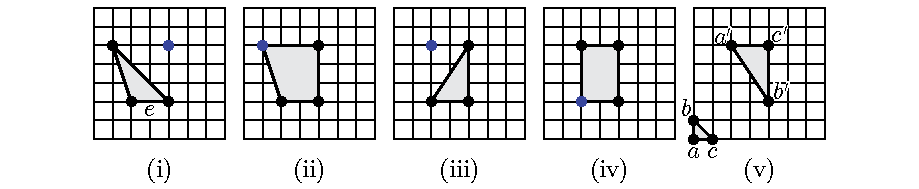
\includegraphics[width=\textwidth]{../assets/connect}
\caption{An illustration of the sequence of deletion and insertion moves from the lattice triangle in (i) to the corner triangle on the bottom-left of (v).}
\label{fig:connect}
\end{center}
\end{figure}
A deletion move on one of the vertices of the quadrilateral then results in a triangle with a horizontal and a vertical edge shown in Fig. \ref{fig:connect}(iii). After that, the triangle has a unique oblique edge that faces one of the four vertices of the square $[0,k]^2$. It is always possible to make this edge face the vertex on the bottom left of the square by performing an insertion move to obtain a rectangle and then a deletion move on the bottom-left vertex of the rectangle. This sequence of moves is illustrated in Figs. \ref{fig:connect}(iii) and \ref{fig:connect}(iv) in the case when the oblique edge initially faces the top left vertex. Finally, one can transform the resulting triangle into the corner triangle of $[0,k]^2$ by inserting the vertices labeled $a$, $b$, and $c$ in Fig. \ref{fig:connect}(v) in this order, the insertion of $x$ being immediately followed by the deletion of $x'$.
\end{proof}

\begin{theorem}\label{lem.Connecd}
For any $d\geq2$ and any positive $k$, $\Gamma(d,k)$ is connected.
\end{theorem}
\begin{proof}
The proof proceeds by induction on $d$. The base case is provided by Theorem \ref{thm.Connec2}. Again, one can always transform a $d$-dimensional lattice $(d,k)$ polytope into a $d$-dimensional simplex by a sequence of deletion moves. Therefore, we only need to prove that the subgraph induced in $\Gamma(d,k)$ by simplices and by polytopes with $d+2$ vertices is connected. The strategy will be, again, to transform any simplex in this graph into the corner simplex of $[0,k]^d$.

Assume that $d\geq3$, consider a lattice simplex $S$ contained in $[0,k]^d$, and call $\mathcal{V}$ the vertex set of $S$. For any $i\in\{1, ..., d\}$, call
$$
\gamma_i^-=\min\{x_i:x\in{S}\}\mbox{ and }\gamma_i^+=\min\{x_i:x\in{S}\}\mbox{.}
$$

Further denote
$$
Q=\prod_{i=1}^d[\gamma_i^-,\gamma_i^+]\mbox{.}
$$

Call $g$ the maximal dimension of the intersection of $S$ and a facet of $Q$. If $g$ is at most $d-2$ then, by Theorem \ref{thm.add}, there exists a facet $R$ of $Q$ such that $S\cap{R}$ is $g$-dimensional and a lattice point $x\in{R}$ such that the convex hull of $S\cup\{x\}$ admits $\mathcal{V}\cup\{x\}$ as its vertex set and the convex hull of $[S\cap{R}]\cup\{x\}$ is a simplex. In other words, one can perform an insertion move on vertex $x$ to transform $S$ into a polytope with vertex set $\mathcal{V}\cup\{x\}$. Since the convex hull of $S\cup\{x\}$ is a simplex, one can find a simplex whose vertex set contains all the vertices of $S\cup\{x\}$, and is a subset of $\mathcal{V}\cup\{x\}$. This simplex can be obtained from the convex hull of $\mathcal{V}\cup\{x\}$ by a single deletion move. Now observe that the intersection of this simplex with $R$ has dimension $g+1$. Repeating this procedure provides a sequence of insertion and deletion moves that transform $S$ into a lattice simplex whose intersection $F$ with a facet $R$ of $Q$ has dimension $d-1$. Call $v$ the unique vertex of the lattice simplex that does not belong to $R$. In other words, this lattice simplex is a pyramid with apex $v$ over $F$. Observe that, in this case, any sequence of insertion and deletion moves that can be performed for $F$ within the cube $\mathrm{aff}(R)\cap[0,k]^d$ can also be performed within $[0,k]^d$ for the pyramid with apex $v$ over $F$. By induction, one can transform $F$ into any lattice simplex in $\mathrm{aff}(R)\cap[0,k]^d$ by a sequence of deletion and insertion moves. Therefore, we can build a sequence of moves that transform $S$ into the $d$-dimensional lattice simplex $S'$ whose vertex set is made up of $v$, of the lattice point $w$ in $\mathrm{aff}(R)\cap[0,k]^d$ with a unique non-zero coordinate, and of the $d-1$ lattice points in $\mathrm{aff}(R)\cap[0,k]^d$ distant by exactly $1$ from $w$.

Now observe that one can perform an insertion move on any lattice vertex distinct from $v$ in the intersection of $[0,k]^d$ with the hyperplane parallel to $R$ that contains $v$. We proceed by inserting the lattice point in this intersection whose orthogonal projection on $R$ is $w$ and then, by deleting $v$. Calling $v'$ any of the $d-1$ lattice points in $\mathrm{aff}(R)\cap[0,k]^d$ distant from $w$ by exactly $1$, the simplex that results from the latter deletion is a pyramid with apex $v'$ over a $(d-1)$-dimensional simplex $F'$ such that, for some $i\in\{1, ..., d\}$, $v'$ satisfies $v'_i=1$ and every vertex $u$ of $F'$ satisfies $u_i=0$. Call $R'$ the facet of $[0,k]^d$ made up of the points $x$ such that $x_i=0$. By induction, one can transform $F'$ within $R'$ into the corner simplex of $R'$. From there, one can perform an insertion move on any lattice vertex distinct from $v'$ in the intersection of $[0,k]^d$ with the hyperplane parallel to $R'$ that contains $v'$. We proceed by inserting the lattice point in this intersection whose orthogonal projection on $R'$ is the origin. Since $v'_i=1$, the $i$-th coordinate of the inserted point is $1$, and its other coordinates are all equal to $0$. Hence, after a last deletion move on $v'$, the resulting simplex is the corner simplex of $[0,k]^d$, as desired.
\end{proof}

\clearpage
\section{Table and Figures}\label{Sec.Tab}

% summary table
\begin{table}[h]
  \begin{center}
  \begin{tabular}{c|r|r|r|r|r|r}
    & \multicolumn{2}{c|}{$1000$ steps} & \multicolumn{2}{c|}{$10000$ steps} & \multicolumn{2}{c}{$100000$ steps} \\
    \hline
    \hline
    $k$ & vertices & volume & vertices & volume & vertices & volume \\
    \hline
    $3$ & $4.798$ & $4.148$ & $4.734$ & 4.353 & 4.711 & 4.343\\
    $4$ & $5.38$ & $7.754$ & $5.288$ & 7.349 & 5.266 & 7.314\\
    $5$ & $6.068$ & $11.844$ & 6.003 & 11.580 & 5.868 & 11.331\\
    $6$ & $6.93$ & $14.934$ & 6.520 & 17.144 & 6.540 & 16.933\\
    $7$ & $7.031$ & $21.050$ & 7.198 & 23.210 & 7.235 & 23.925\\
    $8$ & $7.157$ & $25.922$ & 7.979 & 33.357 & 7.856 & 33.667\\
    $9$ & $8.558$ & $33.712$ & 8.3741 & 44.350 & 8.418 & 41.563\\
    $10$ & $8.736$ & $43.375$ & 8.943 & 55.423 & 9.136 & 56.358\\
    $15$ & $10.483$ & $125.405$ & 11.462 & 101.626 & 11.517 & 137.427\\
    $20$ & $13.07$ & $209.562$ & 14.170 & 219.586 & 13.929 & 246.689\\
    $25$ & $12.695$ & $314.633$ & 15.829 & 376.770 & 16.669 & 374.121\\
    $30$ & $13.501$ & $356.220$ & 16.835 & 532.784 & 18.165 & 585.092\\
    $40$ & $14.904$ & $365.466$ & 20.393 & 714.765 & 22.618 & 855.234\\
    $50$ & $18.875$ & $369.500$ & 21.639 & 816.006 & 25.351 & 1779.055\\
    $60$ & 18.813 & 542.450 & 20.51 & 1112.126 & 27.56 & 2337.680\\
    $70$ & 17.534 & 525.187 & 21.804 & 1271.738 & 31.058 & 3022.452\\
    $80$ & 18.8 & 593.20 & 24.999 & 1547.383 & 32.995 & 3343.108\\
    $90$ & 19.771 & 562.75 & 24.240 & 1499.416 & 33.903 & 3728.283\\
    \hline
  \end{tabular}
  \caption{A summary of measures on the number of vertices and volume of convex polygon visited in a long walk on the Markov chain, for a selection values of $k$ and for $1000$, $10000$ and $100000$ steps walks.}
  \label{Tab.Summary}
  \end{center}
\end{table}

\begin{figure}[h]
  \centering
  \includegraphics[scale=0.7]{npoint_lim}
  \caption{The blue curve shows the verage number of vertices of a polygon in a 1 million steps run, whereas the red one is $2k^{2/3}$.}
  \label{Fig.Nlim}
\end{figure}

\begin{figure}[h]
  \centering
  \includegraphics[scale=0.7]{volume_lim}
  \caption{The blue curve shows the average area of a polygon in a 1 million steps run, whereas the red one is $0.68k^2$.}
  \label{Fig.Vlim}
\end{figure}


\end{document}
